\documentclass[dvisvgm,multi=true]{standalone}
\usepackage{mathmlcoresvg}
\begin{document}
%<figcaption><span>Figure 7: </span>Box model for the <code>mspace</code> element</figcaption>
  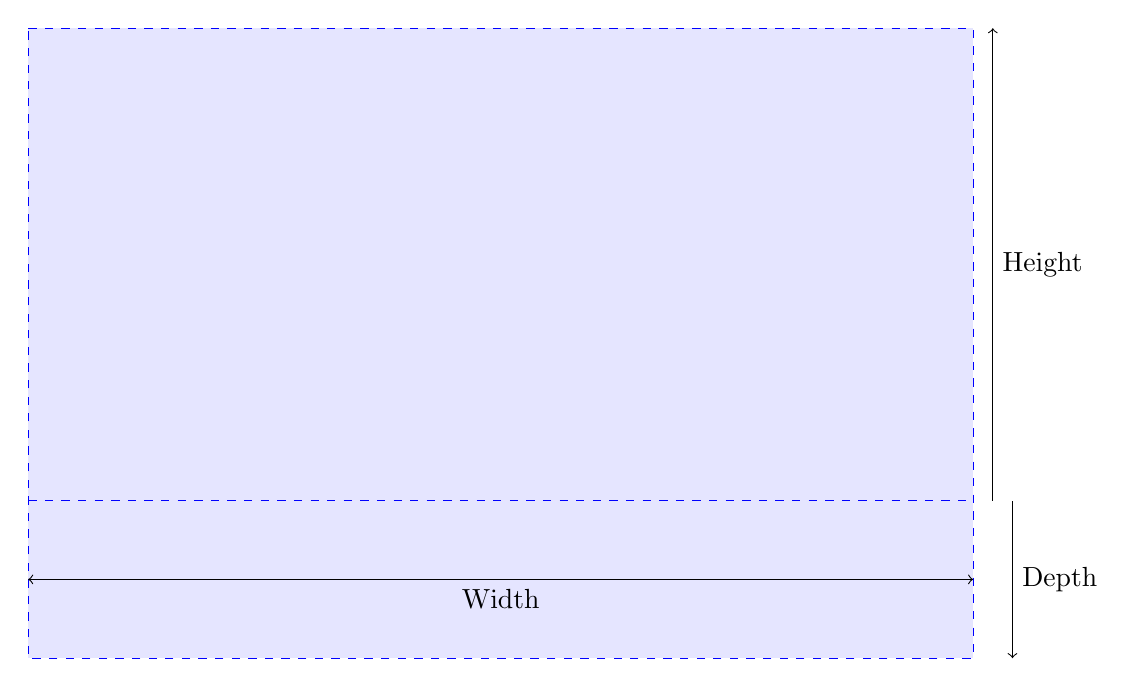
\begin{tikzpicture}[yscale=-1]
  \fill[blue!10] (0,-6) -- (12,-6) -- (12,2) -- (0,2) -- cycle;
  \draw[dashed,blue] (0,-6) -- (12,-6) -- (12,2) -- (0,2) -- cycle
  (0,0)--(12,0);

  \draw[<->] (0,1) -- (6,1) node[below]{Width} -- (12,1);

  \draw[<-] (12.25, -6) --
  (12.25,-3) node[right]{Height} -- (12.25,0);
  \draw[<-] (12.5, 2) --
  (12.5,1) node[right]{Depth} -- (12.5,0);
  \end{tikzpicture}

\end{document}
